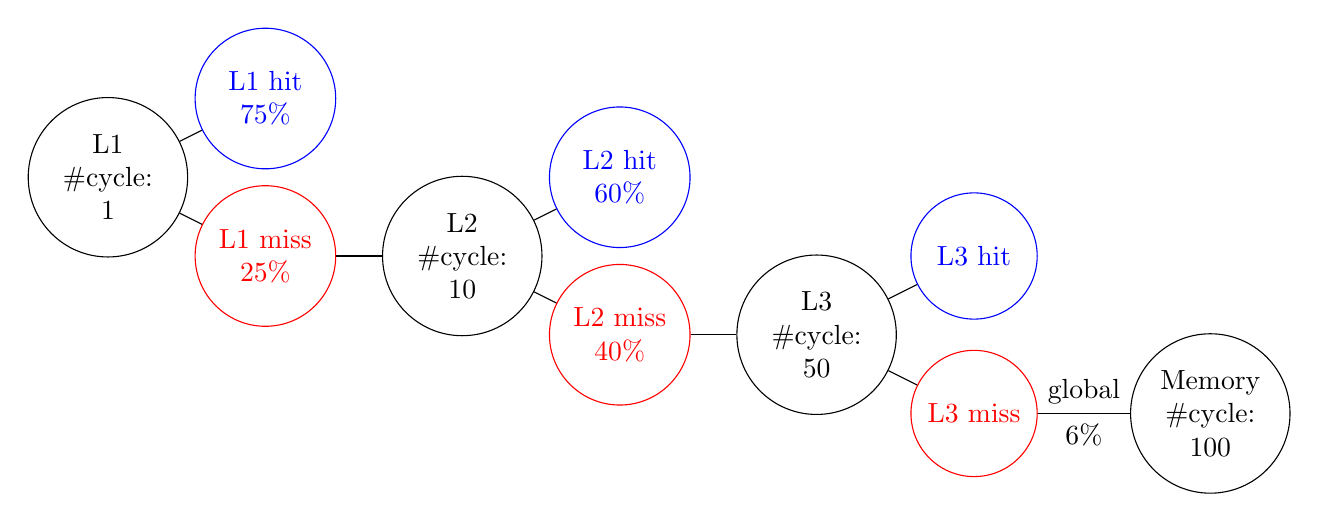
\begin{tikzpicture}
\tikzstyle{s}=[circle, draw, minimum width=1cm,text width=1.3cm,text centered];
\tikzstyle{hit}=[s,blue];
\tikzstyle{miss}=[s,red];
\node [s] (v1) at (-0.5,1) {L1 \#cycle: 1};
\node [hit] (v2) at (1.5,2) {L1 hit 75\%};
\node [miss] (v3) at (1.5,0) {L1 miss 25\%};
\draw  (v1) edge (v2);
\draw  (v1) edge (v3);
\node [s] (v4) at (4,0) {L2 \#cycle: 10};
\draw  (v3) edge (v4);
\node [hit] (v5) at (6,1) {L2 hit 60\%};
\node [miss] (v6) at (6,-1) {L2 miss 40\%};
\draw  (v4) edge (v5);
\draw  (v4) edge (v6);
\node [s] (v7) at (8.5,-1) {L3 \#cycle: 50};
\draw  (v6) edge (v7);
\node [hit] (v8) at (10.5,0) {L3 hit};
\node [miss] (v9) at (10.5,-2) {L3 miss};
\draw  (v7) edge (v8);
\draw  (v7) edge (v9);
\node [s] (v10) at (13.5,-2) {Memory \#cycle: 100};
\draw  (v9) edge node [above] {global} node [below] {6\%} (v10);
\end{tikzpicture}